\section{Grundlagen Flüssigkristalldisplays}
\label{sec:grundlagen_lcd}

\subsection{Aufbau eines Flüssigkristalldisplays}

\begin{figure}[H]
	\centering
	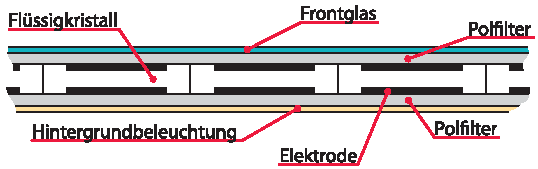
\includegraphics[width=0.75\linewidth]{img/grundlagen/lcd.pdf}
	\caption{Querschnitt eines schwarz-weiß LC Displays}
	\label{fig:lcd_graphic}
\end{figure}

Auf der obigen Skizze dargestellt ist der prinzipielle Aufbau eines LC-Displays. Hinter (\textit{Direct-Lit}) oder neben (\textit{Edge-Lit}) einem Diffusor sitzen LEDs, welche zur Realisierung homogener Hintergrundbeleuchtung verwendet werden. Darüber folgt ein Polfilter, der nur Lichtwellen einer Ausrichtung durchlässt. Das nun gerichtete Licht passiert dann den Flüssigkristall. Dieser Flüssigkristall hat die Eigenschaft die Polarisation des Lichtes je nach anliegender Spannung zu ändern.

Ein weiterer Polfilter hinter diesem Flüssigkristall fungiert als Lichtfilter, da je nach Rotation des Lichtes mehr oder weniger Photonen den zweiten Filter passieren. Wird eine separate Ansteuerung für jeden Pixel realisiert, kann nun ein Bild dargestellt werden.

Für ein Farbdisplay muss jeder Pixel noch in drei Subpixel aufgeteilt werden, von denen jeder einen Farbfilter erhält um nur Licht bestimmter Wellenlänge passieren zu lassen. Eine Standard-Zelle ist die sogenannte TN-Zelle (\emph{T}wisted \emph{N}ematic) und wird in \cite[p.~13]{lcd_lueder} näher beschrieben.

Ein Problem, welches jedoch bei diesem Displaytyp auftritt, ist das sogenannte \emph{Light-Leakage} \cite{light_leakage}, also die nicht einhundert prozentige Absperrung des Pixels, was dazu führt, dass schwarze Grauwerte eines Bildes nicht komplett schwarz erscheinen, sondern einen leichten, oft grau-blauen\cite[p.~71]{light_leakage_color} Schimmer haben (Leuchtdichte\footnote{Im englischsprachigen Raum wird die Leuchtdichte mit der Einheit \emph{nit} beschrieben und entspricht $ \mathrm{\frac{cd}{m^2}} $. } $ \gg 0 \mathrm{\frac{cd}{m^2}} $). Dieses Problem lässt sich mittels \textit{Local-Dimming} mindern, indem in Bereichen, in denen das Bild sehr dunkel ist, die Hintergrundbeleuchtung dunkler oder sogar ganz ausschaltet wird.\\
Die Wahrnehmung elektromagnetischer Strahlung im menschlichen Auge wird mit einer Hellempfindlichkeitskurve, der sogenannten V-Lamda-Kurve auch $ V(\lambda) $, beschrieben. Um von der radiometrischen der Strahldichte zur fotometrischen Leuchtdichte und somit auf die wellenlängenabhängige Wahrnehmungintensität zu gelangen, wird die Strahldichte mit der $ V(\lambda) $ gewichtet.
\begin{figure}[H]
	\centering
	\includegraphics[width=0.75\linewidth]{img/grundlagen/V-lambda-phot-scot}
	\caption{$ V(\lambda) $-Kurve, entnommen aus \cite{v_lambda_IMG}.}
	\label{fig:v-lambda}
\end{figure}

Die blaue Linie stellt hier das Nacht- und die rote Linie das Tagsehen dar. Klar zu erkennen ist, dass das Auge in verschiedenen Wellenlängen verschieden empfindlich ist und somit am Rand des sichtbaren Bereiches eine höhere Strahlungsintensität nötig ist, um die selbe Helligkeitsempfindung zu bewirken wie in der Mitte des sichtbaren Bereiches.\cite{v_lambda}

\subsection{Menschliche Wahrnehmung (Human Visual System)}
\label{subsec:human_visual_system_Gamma}

Das menschliche Auge nimmt Helligkeit nicht linear, sondern annähernd logarithmisch wahr. Dies hat den Vorteil, dass wir mit unseren Augen recht gut Szenen wahrnehmen können, die ein breites Spektrum an Helligkeiten abdecken. Das menschliche Auge kann eine Lichtintensität ($\frac{d \Phi}{d \Omega}$ = $\frac{Energie}{Raumwinkel}$) von 1 bis 10 Millionen wahrnehmen.\cite[p.~33]{light_intensity} \\
Diese sogenannte \textit{Dynamic Range} bedeutet, dass in der unteren Hälfte des Helligkeitsspektrums deutlich mehr Abstufungen erkennbar sind, als im oberen Bereich.

Unter der Annahme, dass die Ansteuerung des Displays linear ist, wäre bei einer 8-bit Ansteuerung der Wert 255 doppelt so energiereich wie 127. Dies wird vom Auge jedoch nicht so wahrgenommen. Da die Wahrnehmung ausschlaggebend ist, die bekanntlich keinen linearen Zusammenhang mit der Leuchtdichte besitzt, wird eine Gamma-Funktion eingeführt, die den Zusammenhang zwischen Wahrnehmung und Leuchtdichte beschreibt. Die Formel für die Gammafunktion lautet
\begin{equation}
L \propto G^\gamma
\end{equation}
wobei $ \gamma $ ein konstanter Wert (typischerweise 2,2) ist. $ L $ entspricht der physikalischen Leuchtdichte, während der Grauwert $ G $ für die Bilddaten verwendet wird. $ G $ wird für dunkle Bereiche höher aufgelöst als für helle Bereiche. Der Grauwert 255 mag dem Betrachter doppelt so hell erscheinen wie der
Grauwert 127. Der Leuchtdichte-Unterschied zwischen den Grauwerten 255 und 127 beträgt jedoch typischerweise Faktor vier.




\begin{figure}[H]
	\centering
	\includegraphics[width=0.75\linewidth]{img/grundlagen/gamma.png}
	\caption{Verschiedene Kurven für verschiedene Werte von Gamma, entnommen aus \cite{gamma_IMG}.}
	\label{fig:gamma}
\end{figure}

\subsection{Dimmen von LEDs}
LEDs lassen sich im Gegensatz zu Glühbirnen nicht über die Spannung dimmen, sondern nur über den Strom, da das Licht proportional zum Strom ist. Eine Stromreglung ist aber elektronisch recht aufwändig zu implementieren, daher wird in der Anwendung meist die sogenannte Pulsweitenmodulation (PWM) verwendet. Zudem hat ein PWM-Betrieb den Vorteil, dass der Farbton des Lichts konstant ist und nicht durch Dimmen geändert wird. \\
Hier werden jedoch beide Techniken vorgestellt.

\subsubsection{Amplitudenmodulation (AM)}
Bei der AM wird der Strom, der durch die LEDs fließen soll, in der Höhe (Amplitude) eingestellt. Eine gängige Methode ist die Regelung der Gate-Spannung des treibenden MOS-Transistors. Ein Vorwiderstand $ R_v $ wird in den Stromkreis eingebaut. Der Spannungsabfall an diesem Widerstand kann gemessen werden ($ U_v=R_v \cdot I_D $). Ist der Spannungsabfall zu hoch und damit auch der LED-Strom, kann die Gate-Spannung reduziert werden. Das gleiche gilt, wenn der Spannungsabfall zu gering ist. \\
Damit der gewünschte Strom $ I_D $ durch die LEDs fließen kann, muss die Versorgungsspannung $ U_0 $ mindestens so groß sein wie die Flussspannung $ U_D $ der Diode bzw. Dioden.
\begin{equation}
U_{0} \geq U_{Dgesamt}=U_{D}\cdot N_{LED}
\end{equation}
$ N_{LED} $ ist die Anzahl der LEDs in einem LED-Strang. Der treibende Transistor und der Vorwiderstand benötigt noch zusätzliche Spannung. Diese zusätzliche Spannung verursacht eine Verlustleistung, die proportional zum LED-Strom ist.\\
Die Amplitudenmodulation ist effektiv ein DC-Betrieb. Möglicher Flickering-Artefakt ist mit dieser Technik ausgeschlossen, allerdings kann sich der Farbton der LED wahrnehmbar mit der Stromamplitude ändern.

\subsubsection{Pulsweitenmodulation (PWM)}
Um den gewünschten Effekt (Helligkeitsänderung) erreichen zu können, muss die LED ganz schnell ein- und ausgeschaltet werden. Hierbei ist es wie beim Film: erfolgt der Wechsel schnell genug, so kann durch die Trägheit des Auges kein Flimmern mehr erkannt werden. 

\begin{figure}[H]
	\centering
	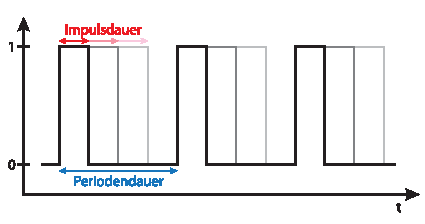
\includegraphics[width=0.5\linewidth]{img/grundlagen/pwm.pdf}
	\caption{Darstellung eines PWM Signals}
	\label{fig:pwm_graph}
\end{figure}

Dieser Graph zeigt drei verschiedene PWM Zyklen mit verschiedenem Dutycycle\footnote{wird auch Tastgrad genannt} (:= Zeit, in der das Signal an ist $ = \tfrac{Impulsdauer}{Periodendauer}$). Je länger das Signal den Wert 1 hat, desto näher ist der Dutycycle an $100\%$.\\

PWM-Signale kommen in der Regel immer dort zum Einsatz, wo ein "`integraler Verbraucher"' (Tiefpass) bedient werden soll. Ein bekanntes Beispiel 
ist die Ansteuerung von elektrischen Maschinen. Sie besitzen eine Induktivität, in der sich der Strom nach 
\begin{align*}
I=\frac{1}{L} \cdot \int_{t}U(t)dt
\end{align*}
berechnet bzw. einstellt. 
Somit kann über ein PWM-Signal die Spannung so gepulst werden, dass sich die gewünschte Stromfunktion in der Induktivität "`einstellt"' (Erklärung nur 
rudimentär). In unserem Fall ist der "`integrale Verbraucher"' das menschliche Auge.  Mittels des PWM-Signals wird der Ladungsfluss (Strom) der LEDs über die Zeit gesteuert, d.h., dass die Amplituden von Spannung und Strom konstant bleiben.
Weiterhin ist das PWM-Signal periodisch mit Periodendauer T. Die Pulslänge (Duty-Cycle) ist ein prozentualer Anteil der Periodendauer T (Abbildung \ref{fig:pwm_graph}). 

Um auf die Anfangsfrage der LED-Dimmung zurück zu kommen folgt, dass der LED-Strom eine gepulste Stromfunktion ist. Aufgrund des "`integralen Verbrauchers"' wird jedoch nur der Mittelwert des Stromes 
und damit der Helligkeit wahrgenommen. Um das PWM-Signal auf den LED-Strom abzubilden, wird ein Transitor (MOSFET) als Schalter in den 
LED-Stromkreis eingefügt. Dieser geht bei einem High-Pegel am Gate (NMOS) in den leitenden Zustand über und es kann ein Strom durch die LEDs fließen. 
Bei einem Low-Pegel am Gate des MOSFET geht dieser in den nichtleitenden Zustand über und der Stromfluss wird unterbrochen (Betrachtung des Transistors als 
idealer Schalter). Um nun die Amplitude des Stromes einzustellen, werden wieder die zur Verfügung stehende Spannung $U_{v}$ und der gewünschte maximale
Strom $I_{Dmaximal}$ betrachtet.

Durch das Verhältnis von Puls"=zu"=Periodendauer des PWM-Signals stellen sich
die Stromfunktion und der wahrgenommene Mittelwert der Helligkeit ein.
\pagebreak

\subsection{\textsc{Versuch 1 und Aufgaben}}
Siehe Dokument zur Aufgabenstellung Kapitel 1.